\documentclass{article}
\usepackage{tikz}
\usetikzlibrary{shapes, positioning, fit, backgrounds, arrows.meta}

\begin{document}
\begin{figure}[htbp]
\centering
\vspace{1cm}
\resizebox{\textwidth}{!}{
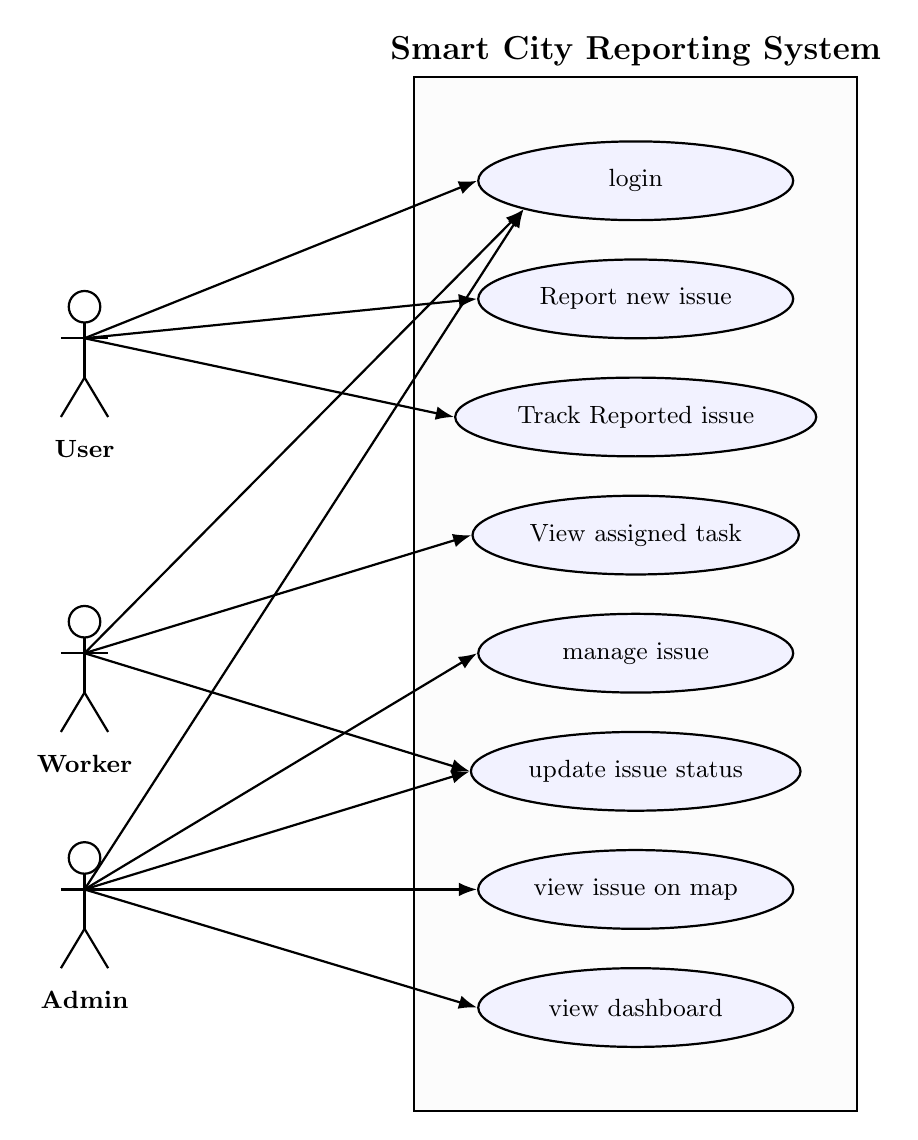
\begin{tikzpicture}[
    >=Latex, thick,
    actor/.style={align=center, font=\small\bfseries},
    usecase/.style={draw, ellipse, minimum width=4cm, minimum height=1cm, align=center, fill=blue!5, font=\small}
]

% -------------------------
% Custom Stickman Definition
% -------------------------
\tikzset{
    stickman/.pic={
        \coordinate (-chest) at (0, 0);
        \draw[thick] (0, 0.4) circle (0.2); % Head
        \draw[thick] (0, 0.2) -- (0, -0.5); % Body
        \draw[thick] (-0.3, 0) -- (0.3, 0); % Arms
        \draw[thick] (0, -0.5) -- (-0.3, -1); % Left Leg
        \draw[thick] (0, -0.5) -- (0.3, -1); % Right Leg
    }
}

% -------------------------
% Use Cases (Center Column inside Boundary)
% -------------------------
\node[usecase] (UC1) at (0, 6) {login};
\node[usecase] (UC2) at (0, 4.5) {Report new issue};
\node[usecase] (UC3) at (0, 3) {Track Reported issue};
\node[usecase] (UC4) at (0, 1.5) {View assigned task};
\node[usecase] (UC5) at (0, 0) {manage issue};
\node[usecase] (UC6) at (0, -1.5) {update issue status};
\node[usecase] (UC7) at (0, -3) {view issue on map};
\node[usecase] (UC8) at (0, -4.5) {view dashboard};

% -------------------------
% System Boundary Envelope
% -------------------------
\begin{scope}[on background layer]
    % Surrounds all use cases cleanly
    \node[draw, rectangle, thick, fill=gray!2, inner sep=0.8cm, fit=(UC1) (UC8)] (System) {};
    % Title at the very top of the bounding box
    \node[anchor=south, font=\large\bfseries] at (System.north) {Smart City Reporting System};
\end{scope}

% -------------------------
% Actors Definition
% -------------------------

% 1. User Actor (Top)
\pic (UserPic) at (-7, 4) {stickman};
\node[actor] (UserLabel) at (-7, 2.6) {User};

% 2. Worker Actor (Middle) -> ADDED AS PER INSTRUCTIONS!
\pic (WorkerPic) at (-7, 0) {stickman};
\node[actor] (WorkerLabel) at (-7, -1.4) {Worker};

% 3. Admin Actor (Bottom)
\pic (AdminPic) at (-7, -3) {stickman};
\node[actor] (AdminLabel) at (-7, -4.4) {Admin};


% -------------------------
% Association Paths (Matching EXACT arrow style from screenshot)
% -------------------------

% User Links
\draw[->] (UserPic-chest) -- (UC1.west);
\draw[->] (UserPic-chest) -- (UC2.west);
\draw[->] (UserPic-chest) -- (UC3.west);

% Worker Links
\draw[->] (WorkerPic-chest) -- (UC1.south west); % Unified login access
\draw[->] (WorkerPic-chest) -- (UC4.west);
\draw[->] (WorkerPic-chest) -- (UC6.west);

% Admin Links
\draw[->] (AdminPic-chest) -- (UC1.south west); % Unified login access
\draw[->] (AdminPic-chest) -- (UC5.west);
\draw[->] (AdminPic-chest) -- (UC6.west);
\draw[->] (AdminPic-chest) -- (UC7.west);
\draw[->] (AdminPic-chest) -- (UC8.west);

\end{tikzpicture}
}
\caption{Use Case Diagram mapped directly to physical hand-drawn entities plus unified Worker flow}
\end{figure}
\end{document}

